% Template for ICASSP-2016 paper; to be used with:
%          spconf.sty  - ICASSP/ICIP LaTeX style file, and
%          IEEEbib.bst - IEEE bibliography style file.
% --------------------------------------------------------------------------
\documentclass[12pt]{article}
\usepackage{spconf, amsmath, graphicx, float}
\usepackage{scrlayer-scrpage}
\clearpairofpagestyles
\cfoot*{\pagemark}
% Example definitions.
% --------------------
\def\x{{\mathbf x}}
\def\L{{\cal L}}

% Title.
% ------
\title{Lending Club Default Probability Prediction}
%
% Single address.
% ---------------
\name{Atom Group: Jifu Zhao (jzhao59), Jinsheng Wang (jwang278)}
\address{Nuclear, Plasma, and Radiological Engineering \\
              University of Illinois at Urbana-Champaign\\
		       Urbana, Illinois 61801, USA}

\begin{document}
%\ninept
%
\maketitle

\section{Introduction}
\quad\ In this project, our goal is to build a model to predict the chance of default for a loan with historical data collected through the Lending Club. The original data set has more than 1,3000,000 records (from 2007 to 2016) and each record has 74 features. In this project, we first do some visualization work to explore the given data set, ino order to have a sense of what the data looks like. After some tricky data cleaning and pre-processing steps, we applied several different Machine Learning models to predict the chance of default for a given loan. More details will be described in the following sections.

\section{Data Pre-processing}
\quad After exploring the whole data set, we noticed that there are 74 features in total. Among these 74 features, we first dropped feature $id$ and $member\_id$ for they are obviously useless. Among other features, we found that features contains high percentage of missing values, so we dropped these below features as well.\\ 

$mths\_since\_last\_delinq$, $ max\_bal\_bc $, $ all\_util $, $ total\_cu\_tl $, $ mths\_since\_last\_record$, \\$ mths\_since\_last\_major\_derog $, $ annual\_inc\_joint $, $ dti\_joint $, $ open\_acc\_6m $, $ open\_il\_6m $, $ inq\_last\_12m $, $ open\_il\_12m $, $ open\_il\_24m $, $ il\_util $, $ inq\_fi $, \\$ mths\_since\_rcnt\_il $, $ total\_bal\_il $, $ open\_rv\_12m $, $ open\_rv\_24m $ \\


In addition to these above deleted features, we again removed some useless features judging from common sense or logic listed as below.\\

$emp\_title$, $issue\_d$, $pymnt\_plan$, $url$, $desc$, $title$, $zip\_code$, $addr\_state$, $earliest\_cr\_line$, \\$last\_pymnt\_d$, $next\_pymnt\_d$, $last\_credit\_pull\_d$, $application\_type$, $verification\_status\_joint$, \\$grade$, $policy\_code$.\\ 

Futhermore, since the order of $sub\_grade$ represents some extent of a loaner's credit, which will surely affect the chance of default, we directly transform this feature into numerical values. After that, for the small portion of missing values in remaining numerical features, we fill them with the median of the corresponding feature in the whole training set. Lastly, the dependent feature, also known as outcome variable, $loan\_staus$, was transformed into 0-1 binary values for later classification algorithms.

    After the above procedures, there are 36 features left. Among these 36 features, there are 30 numerical features and 6 categorical features. For categorical features, we transform them into dummy variables. Within these numerical features, for those whose skewness is above 0.75, we applied log transformation for better gaussian like distribution. After all of these steps, we have well prepared the data set. Then followed the instructions we splitted it into 3:1 training vs. testing data subsets. Training set was used for classifier construction while testing set examined the good and bad of these classifiers.

In our R code, we loaded 6 libraries to simplify our task, including xgboost, randomForest, gbm, dummies, DAAG, glmnet.


\section{Methods}

\subsection{Logistic Regression}
\quad In our first model, Model 1, we basically throwed all the features we have created above into the logistic regression algorithm and performed the easiest glm method in "glmnet" library as a benchmark for comparison with more advanced algorithms later. This model is easy and fast, though the performance may not be good compared with other methods.

\subsection{Random Forest}
\quad In our second model, Method 2, we deployed Random Forest algorithm to tackle this classification problem. In this algorithm, there are several parameters need to be tuned in order to get the best of the algorithm. Random Forest in itself sampled m features out of p features when building tree nodes. Large number of trees together can solve the high vaiance of each tree, thus giving this algorithms power to deal with low bias but high variance problem of decision trees. In our project, after tiral and error based on the plot of errors vs. number of trees, we found that 200 tress would be sufficient. But during testing, 300 trees was used to guarantee the performance. Also, in the whole data set, only 7\% data is labeled with 1 (defalut loan). This unbalanced problem was resolved by sampling 100 1's and 100 0's each time when building each classifier tree. Besides, feature importance was set to be TRUE thus the algorithms will automatically choose the best m within p features. Random Forest was more computation intensive, costing longer CPU time but  gave out better result than simple Logistic Regression above.

\subsection{XGBoost}
\quad In our third, also the last model, Method 3, we called XGBoost algorithm to conquer the problem. XGBoost is an across platform, multi-interface supported implementation of gradient boosted decision trees designed for high speed and better perfomance. Also, there are several parameters we can adjust to maximize the power of XGBoost algorithm, they are tree depth max.depth (6 in our case), learning rate eta (0.3 in our case), the number of round for boosting nround (100 in our case) , unbalanced data ratio as num(0):num(1) $ scale\_pos\_weight $ (calculated by this ratio for each training set, around 13). XGBoost used less time while achived better result than that of RandomForest, showing the power and advantage of this algorithm.


\section{Code Description}
\quad\ All of our code is contained in the file named mymain.R. 

There are basically three parts in the R file. At the very beginning, the code will automatically check whether or not the required packages/libraries are already installed. In the second part of the code, we do data preprocessing: first read the training and test data sets, then drop the useless variables and process the features to form the new feature space. For the last part, we mainly build our three model: Logistic Regression, Random Forest model and XGBoost model. These built models will make predictions and the results are saved into local file system as required by the project description.

Due to the amount of data to be looped, the code need a lot of time to run. As tested, the total running time is around 70 mins.

\section{Results}

\quad To evaluate our model, we choose the metric described on Kaggle:
\begin{equation}
logloss = - \frac{1}{N} \sum_{i=1}^N \sum_{j=1}^M y_{i, j} log(p_{i, j})
\end{equation}
where $N$ is the number of test cases, $M$ is the total classification classes. To avoid the problem where $p_{i, j} = 0$, we scale $p_{i, j}$ into $10 ^ {-15}$ and $1 - 10 ^ {-15}$.


\begin{table}[htb]
 \caption{Summary of Training Loss} \label{result}
 \vspace{0.1in}
\begin{center}
  \begin{tabular}{  c  c  c  c  c}
    \hline
    Split            & Seed        & Model 1    & Model 2    & Model 3 \\ \hline
    Split 1         & 100    &0.0721    &0.0255    &0.0163\\ \hline
    Split 2         & 500    &0.0714    &0.0252    &0.0161\\ \hline
    Split 3         & 1000    &0.0713    &0.0254    &0.0165\\ \hline
    Split 4         & 5000    &0.0718    &0.0254    &0.0165\\ \hline
    Split 5         & 2017    &0.0712    &0.0253    &0.0161\\ \hline
  \end{tabular}
\end{center}
\end{table}
\begin{table}[htb]
 \caption{Summary of Test Loss} \label{result}
 \vspace{0.1in}
\begin{center}
  \begin{tabular}{  c  c  c  c  c}
    \hline
    Split            & Seed        & Model 1    & Model 2    & Model 3 \\ \hline
    Split 1         & 100    &0.0693    &0.0248    &0.0202\\ \hline
    Split 2         & 500    &0.0724    &0.0256    &0.0212\\ \hline
    Split 3         & 1000    &0.0729    &0.0259    &0.0211\\ \hline
    Split 4         & 5000    &0.0709    &0.0251    &0.0202\\ \hline
    Split 5         & 2017    &0.0730    &0.0255    &0.0208\\ \hline
  \end{tabular}
\end{center}
\end{table}


From Table~\ref{result}, one can find that, model 1 (Logistic Regression) performed stable results for training and testing, but worest among all three models. Model 2 (Random Forest) gave out stable results for both training and testing, and also better than that of model 1. Model 3 (XGBoost) had the lowest training and tesing error, but the former one is kind of lower than that of the latter, suggesting possiblely slight over fitting.


The above code was tested on our own laptop, the average running time is about 1.5 hours. The corresponding computer system is:
MacBook Pro, 2.6GHz Intel Core i7, 16 GB memory.  

\subsection*{Acknowledgement}

%\begin{figure}[htb]
%\centering
%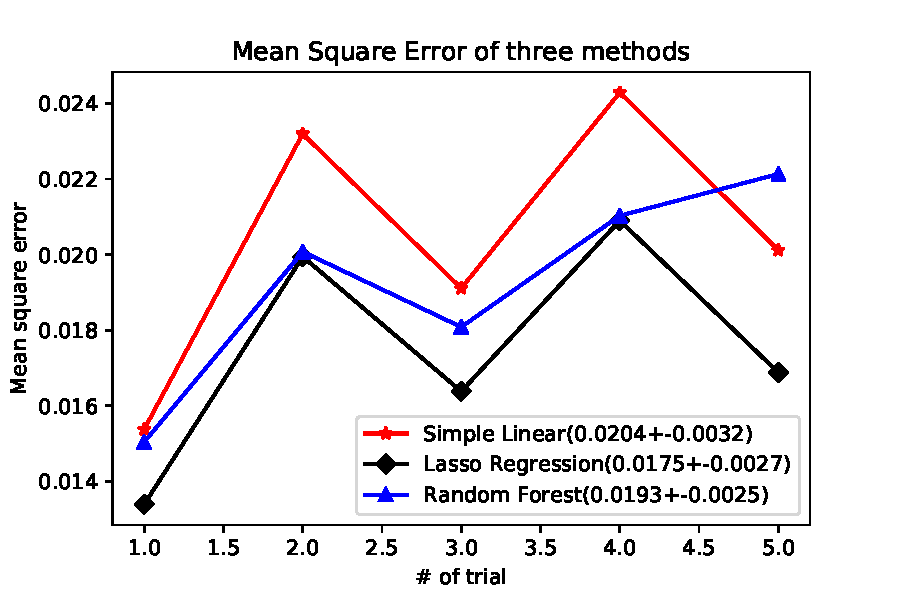
\includegraphics[width=0.45\textwidth]{./figures/MSE_3_methods.pdf}
%\caption{Results of different models}
%\label{fig:autoencoder}
%\end{figure}

\quad\ The authors would like to thank Xichen Huang for his tutorial notebook on Piazza.

\vfill\pagebreak

% References should be produced using the bibtex program from suitable
% BiBTeX files (here: strings, refs, manuals). The IEEEbib.bst bibliography
% style file from IEEE produces unsorted bibliography list.
% -------------------------------------------------------------------------
%\bibliographystyle{IEEEbib}%\bibliography{strings,refs}
%\bibliography{strings}

\end{document}